\documentclass{beamer}
\mode<presentation>
\usepackage{tikz}
\usepackage{multimedia}
\setbeamertemplate{caption}{\insertcaption}
\renewcommand{\thefootnote}{\fnsymbol{footnote}}
% \usepackage{pdfpc-movie}
\usepackage{graphicx} %The mode "LaTeX => PDF" allows the following formats: .jpg  .png  .pdf  .mps
% \usepackage{media9}
\usetikzlibrary{arrows, shapes.geometric,matrix,positioning,graphs,quotes}
\title{Computational Thinking in Science Curriculum}
\author[dishajk]{Disha Kuzhively}
\institute{International Centre for Theoretical Sciences - TIFR, Bangalore}
\date[Chennai]{Pre-Orientation Workshop on Curriculum Framing and Syllabus Preparation for Science and Mathematics\\\today\\{\texttt disha.jk@icts.res.in} }
\begin{document}
\begin{frame}
    \titlepage
\end{frame}
\begin{frame}
    \frametitle{Outline}
    \tableofcontents
\end{frame}
\section{Introduction}
\begin{frame}
Computational thinking is a set of problem-solving methods that involve expressing problems and their solutions in ways that a computer could also execute.
\end{frame}

\section{Example: Conditional Statement - If Then Else}

\begin{frame}
  \frametitle{4 S2 III Transparent,Translucent and Opaque objects}
  \only<1>{
    \includegraphics[width=0.65\textwidth]{opacity-102.png}
    \includegraphics[width=0.65\textwidth]{opacity-103.png}
  }
  \only<2>{

  \begin{block}{Exercise}
    Classify the objects given below as transparent, translucent or opaque materials. 
    
    Air, Rock, Water, Aluminium foil, Mirror, Snow, Wooden board, Polythene bag, CD, Oil soaked paper, Glass tumbler and Coloured glass
  \end{block}
  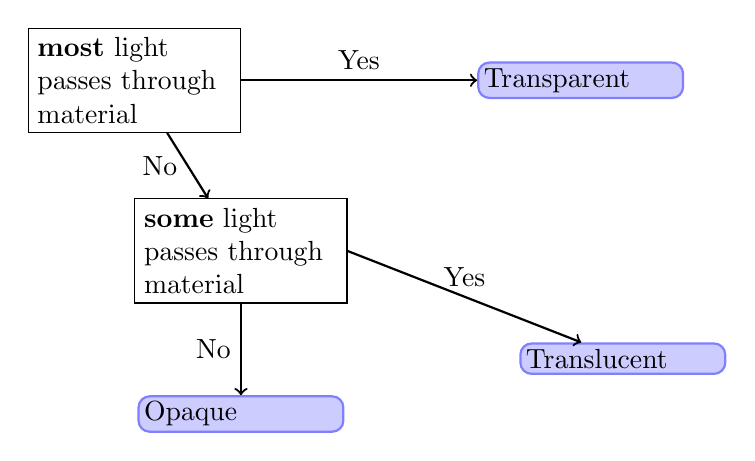
\begin{tikzpicture}[final/.style={draw=blue!50,fill=blue!20,thick,inner sep=2pt, rounded corners}]
    \node[rectangle, draw, text width=7em, anchor=east] (a) at (0,0) {{\bfseries most} light passes through material};
    \node[rectangle, draw, text width=7em,anchor=west,] (b) at (0:3) [final]{Transparent};
    \draw[->,thick] (a) -- node[midway, above] {Yes} (b);
    \node[rectangle, draw, text width=7em,anchor=north] (c) at (-90:1.5) {{\bfseries some} light passes through material};
    \draw[->,thick] (a) -- node[midway, left] {No} (c);
    \node[rectangle, draw, text width=7em,anchor=west,] (d) at (-45:5) [final]{Translucent};
    \draw[->,thick] (c.east) -- node[midway, above] {Yes} (d);
    \node[rectangle, draw, text width=7em,anchor=north] (e) at (-90:4) [final]{Opaque};
    \draw[->,thick] (c.south) -- node[midway, left] {No} (e);
  \end{tikzpicture}
  }
\end{frame}
\begin{frame}
  \frametitle{6.3.6 Separation of Mixtures}
  \only<1>{
  \includegraphics[height=\textheight]{mixtures-048.png}}
  \only<2>{
  Separating mixture containing solid and liquid

  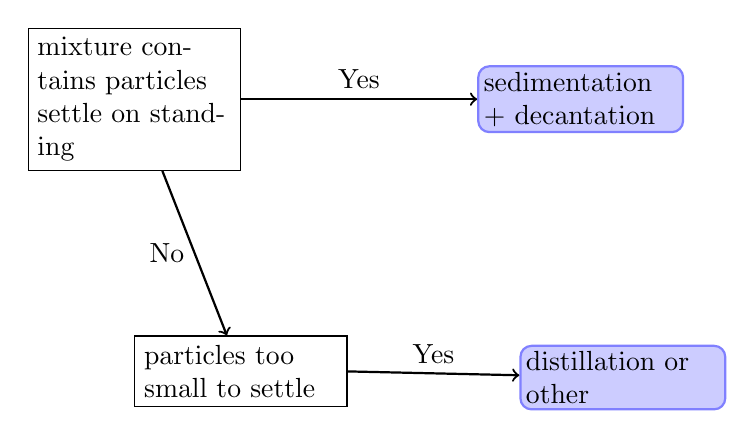
\begin{tikzpicture}[final/.style={draw=blue!50,fill=blue!20,thick,inner sep=2pt, rounded corners}]
    \node[rectangle, draw, text width=7em, anchor=east] (a) at (0,0) {mixture contains particles settle on standing};
    \node[rectangle, draw, text width=7em,anchor=west,] (b) at (0:3) [final]{sedimentation $+$ decantation};
    \draw[->,thick] (a) -- node[midway, above] {Yes} (b);
    \node[rectangle, draw, text width=7em,anchor=north] (c) at (-90:3) {particles too small to settle};
    \draw[->,thick] (a) -- node[midway, left] {No} (c);
    \node[rectangle, draw, text width=7em,anchor=west,] (d) at (-45:5) [final]{distillation or other};
    \draw[->,thick] (c.east) -- node[midway, above] {Yes} (d);

  \end{tikzpicture}}
\end{frame}


\begin{frame}
  \frametitle{If-Then-Else Flow Diagram}
  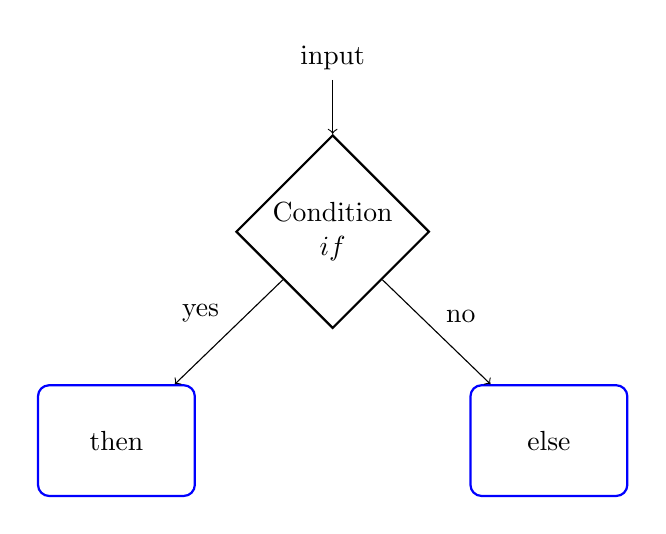
\begin{tikzpicture}[ampersand replacement=\&,auto,
  decision/.style={diamond,draw,thick,text width=4.5em,align=flush center,inner sep=1pt},
  block/.style={rectangle, draw=blue, thick, text width=5em,align=center, rounded corners,minimum height=4em},
  line/.style={draw, thick, -latex',shorten >=2pt}]
  
  \matrix [column sep=5mm,row sep=7mm]{
    \& \node (input) {input}; \& \\
    \& \node [decision] (if) {Condition\\\(if\)}; \& \\
    \node [block] (then) {then}; \& \& \node [block] (else) {else};\\
  };
  \graph {(input)->(if)};
  \graph[edge label'=yes] {(if)->(then)};
  \graph[edge label=no] {(if)->(else)};
  \end{tikzpicture}

\end{frame}
\section{Example: Cooling of Water}
\begin{frame}
  
  \begin{columns}
    \begin{column}{0.45\textwidth}
      \only<1-2>{
\includegraphics[width=\textwidth]{linear-graph.png}
      }
      \only<3>{
\includegraphics[width=0.8\textwidth]{cooling.jpg}
      }
    \end{column}
    \begin{column}{0.55\textwidth}
      \uncover<2-3>{
         \includegraphics[width=\textwidth]{temp-time.png}
      }
    \end{column}
  \end{columns}
\end{frame}
\section{Example: Loop Iteration}
\begin{frame}
  \frametitle{Kerala SCERT Class 7, 8. Wonders of the Sky}
  how many days it takes for the Moon to reach the New Moon from Full Moon?

  \begin{tikzpicture}
    \draw (0,0) grid (5,5);
    \node[anchor=south west] (image) at (0,0) {\includegraphics[width=0.6\textwidth]{moon-53.png}};
    \only<2-3>{
      \node[xshift=4em,yshift=2em, text width =10em] at (image.east) {1. Identify full-moon date; 2. Identify next new-moon date; 3. Compute difference; 4. Repeat for next month.};
    }
    \only<3>{\node[xshift=4em,text width =8em,blue!50!black] at (image.south east) {Decompposition/ Defining subroutines/ functions};}
    \only<4>{
      \node[xshift=4em, text width =10em] at (image.east) {Detecting regularities e.g. loop iteration count or periodicity in data.
      
      Algorithm $\to$ Follows a clear sequence: find full-moon date $\to$ find next new-moon date $\to$ subtract $\to$ record $\to$ repeat for next month.};
    }
  \end{tikzpicture}
\end{frame}
\section{How to Identify Computational Thinking Moments in the Science Textbooks?}
\begin{frame}
  \frametitle{Computational Thinking Moments in the Science Textbooks}
  \begin{itemize}
  \item<1-> Understanding the problem
  \item<2-> \alert{Decomposition}: break down a complex problem into manageable sub-problems.
  \item<3-> Plan a method, design an experiment/solution, sequence actions: \alert{Algorithm}
  \item<4-> Abstraction and pattern recognition, focusing on relevant features.
  \only<4>{Tasks requiring comparison of data, drawing tables/graphs, identifying patterns, generalising from data, ignoring irrelevant detail}
  \item<5-> Testing, debugging, evaluation
  \only<5>{test the solution, reflect on limitations, verify fairness of test}
  \item<6-> Data visualisation
  \only<6>{Use of charts/tables/graphs to represent results}
\end{itemize}
\end{frame}
\begin{frame}
  \begin{tikzpicture}
  \node (polya1) at (0,0) {\includegraphics[height=0.45\textheight]{polya1.png}};
  \node (polya2) at (0,-0.5*\textheight){\includegraphics[height=0.45\textheight]{polya2.png}};
  \draw[->] (polya2.south east) to [out=0,in=0] (polya1.east);
  \end{tikzpicture}
\end{frame}
\end{document}
